\section{Proof of the forest estimate}\label{sec:forest}

This section proves Theorem~\ref{thm:forest}. The argument is that of~\cite{KNT}. It has five steps.
\begin{enumerate}
\item \emph{Cuts.} For a set $A$ of vertices, consider the event that $\xi$ avoids every edge that
leaves $A$. Its probability is explicit. For two disjoint sets the two events are correlated by the
factor $2^{\ell-1}$, where $\ell$ counts the links between the sets (Lemma~\ref{lem:link}). One link
means independence, and two links mean a factor of two.
\item \emph{Reduction.} We pass to a graph $\Gamma$ with all degrees at most $3$, in which $W$ has
become a small set $P$ of vertices (Lemma~\ref{lem:reduce}).
\item \emph{Short cycles.} Step~1 and a second moment bound show that many disjoint short cycles in
$\Gamma-P$ already force the estimate (Lemma~\ref{lem:smallcuts}). So we may delete a small maximal
family of them, and we are left with a graph $J$ of large girth.
\item \emph{Supply.} The graph $J$ has many cycles with between $6\log r$ and
$\log r\sqrt{\log\log r}$ edges. Their total weight $\sum_C2^{-|C|}$ is at least
$(\frac18-o(1))\ln\log\log r$ (Lemma~\ref{lem:weight}). This step uses the non-backtracking matrix.
\item \emph{Second moment.} For such a cycle $C$, the event that $C$ is a component of $\xi$ has
probability at least $2^{-|C|}$. If it occurs, then the part of $\xi$ outside $P$ is not a forest.
We weight the indicators of these events so that their means are exactly $2^{-|C|}$. Most pairs of
the events are correlated by a factor of at most two.
\end{enumerate}
The factor two in step~5 is the source of the constant $\half$. Lemma~\ref{lem:second} turns the
bound $\EE Z^{2}\le2\mu^{2}+K\mu$ into $\PP(Z=0)\le\half+K/(4\mu)$. Appendix~\ref{app:lean} lists the
Lean declarations that correspond to the steps.

In this section graphs may have loops and parallel edges. A loop adds two to the degree of its vertex
and is a cycle of length one. Two parallel edges form a cycle of length two. For a set $A$ of
vertices of $G$ we write $G[A]$ for the induced subgraph, $G-A$ for $G[V(G)\sm A]$, and $\delta A$
for the set of edges with exactly one end in $A$. A \emph{region} is a nonempty set $A$ such that
$G[A]$ is connected. A region is \emph{cyclic} if $G[A]$ contains a cycle. As before $\xi$ is
uniform on $\Z(G)$, and $\cO_A$ denotes the event $\xi\cap\delta A=\emptyset$.

\subsection{Cuts and links}

\begin{lemma}\label{lem:second}
Let $Z\ge0$ be a random variable with $\mu=\EE Z>0$ and $\EE Z^{2}\le2\mu^{2}+K\mu$. Then
$\PP(Z=0)\le\half+K/(4\mu)$.
\end{lemma}

\begin{proof}
By the Cauchy--Schwarz inequality $\mu^{2}\le\EE Z^{2}\cdot\PP(Z>0)$, so
$\PP(Z=0)\le1-\mu/(2\mu+K)\le\half+K/(4\mu)$.
\end{proof}

Let $A$ and $B$ be disjoint regions of a connected graph $G$. A \emph{link} between them is an edge
with one end in $A$ and the other in $B$, or a component of $G-(A\cup B)$ that is joined by an edge
to $A$ and by an edge to $B$ (Figure~\ref{fig:links}). Let $\ell(A,B)$ be the number of links.

\begin{figure}[ht]
\centering
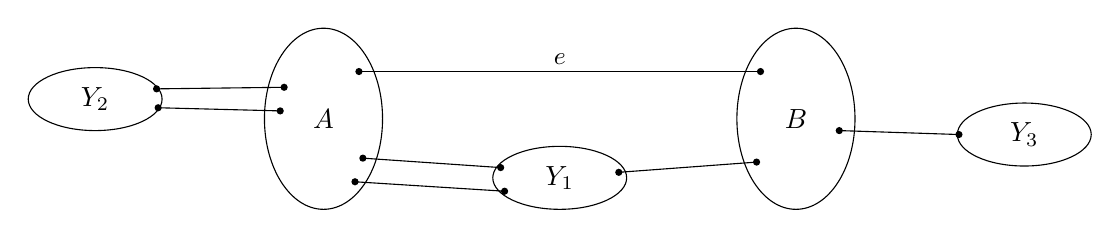
\begin{tikzpicture}
  \draw (0,0) ellipse [x radius=0.75, y radius=1.15];
  \draw (6,0) ellipse [x radius=0.75, y radius=1.15];
  \draw (3,-0.75) ellipse [x radius=0.85, y radius=0.4];
  \draw (-2.9,0.25) ellipse [x radius=0.85, y radius=0.4];
  \draw (8.9,-0.2) ellipse [x radius=0.85, y radius=0.4];
  \node at (0,0) {$A$};
  \node at (6,0) {$B$};
  \node at (3,-0.75) {$Y_1$};
  \node at (-2.9,0.25) {$Y_2$};
  \node at (8.9,-0.2) {$Y_3$};
  \draw (0.45,0.6) -- node[above=-1pt] {\small$e$} (5.55,0.6);
  \draw (0.5,-0.5) -- (2.25,-0.62);
  \draw (0.4,-0.8) -- (2.3,-0.92);
  \draw (5.5,-0.55) -- (3.75,-0.68);
  \draw (-0.5,0.4) -- (-2.12,0.38);
  \draw (-0.55,0.1) -- (-2.1,0.14);
  \draw (6.55,-0.15) -- (8.07,-0.2);
  \foreach \p in {(0.45,0.6),(5.55,0.6),(0.5,-0.5),(2.25,-0.62),(0.4,-0.8),(2.3,-0.92),(5.5,-0.55),
                  (3.75,-0.68),(-0.5,0.4),(-2.12,0.38),(-0.55,0.1),(-2.1,0.14),(6.55,-0.15),(8.07,-0.2)}
    \fill \p circle (1.3pt);
\end{tikzpicture}
\caption{Links between two regions $A$ and $B$. The edge $e$ and the component $Y_1$ of
$G-(A\cup B)$ are links. The components $Y_2$ and $Y_3$ are joined to one region only, so they are
not links. Here $\ell(A,B)=2$. In the proof of Lemma~\ref{lem:link} this is the case $a=b=k=1$
and $e(A,B)=1$.}
\label{fig:links}
\end{figure}

\begin{lemma}[Link formula]\label{lem:link}
Let $A$ and $B$ be disjoint regions of a connected graph $G$. Then
$\PP(\cO_A)=2^{\comp(G-A)-|\delta A|}\ge2^{-|\delta A|}$ and
\[
  \PP(\cO_A\cap\cO_B)=2^{\ell(A,B)-1}\,\PP(\cO_A)\,\PP(\cO_B).
\]
Conditionally on $\cO_A$, the set $\xi\cap E(G[A])$ is uniform on $\Z(G[A])$; conditionally on
$\cO_A\cap\cO_B$, the sets $\xi\cap E(G[A])$ and $\xi\cap E(G[B])$ are independent and uniform on
$\Z(G[A])$ and $\Z(G[B])$.
\end{lemma}

\begin{proof}
The even subgraphs that avoid $\delta A$ are the sums of an even subgraph of $G[A]$ and an even
subgraph of $G-A$. So $\PP(\cO_A)=2^{\beta(G[A])+\beta(G-A)-\beta(G)}$, and counting edges and
vertices shows that the exponent is $\comp(G-A)-|\delta A|$. In the same way
\[
  \PP(\cO_A\cap\cO_B)=2^{\beta(G[A])+\beta(G[B])+\beta(G-A-B)-\beta(G)}
     =2^{\comp(G-A-B)+1-|\delta A|-|\delta B|+e(A,B)},
\]
where $e(A,B)$ is the number of edges between $A$ and $B$. Let $a$, $b$ and $k$ be the numbers of
components of $G-A-B$ that are joined to $A$ only, to $B$ only, and to both. Then
$\comp(G-A-B)=a+b+k$, while $\comp(G-A)=a+1$ and $\comp(G-B)=b+1$, and the formula follows since
$\ell(A,B)=k+e(A,B)$. The conditional laws are read off from the two direct sum decompositions.
\end{proof}

So two cut events are independent when there is one link. They are correlated by a factor of
exactly two when there are two links. The correlation is stronger only for pairs with at least
three links, and the next lemma says that such pairs are rare.

\begin{lemma}[Exceptional partners]\label{lem:exc}
Let $A$ be a region of a connected graph $G$, and let $B_1,\dots,B_k$ be pairwise disjoint regions,
disjoint from $A$, with $\ell(A,B_i)\ge3$ for all $i$. Then $k\le|\delta A|$.
\end{lemma}

\begin{proof}
Contract $A$ to a vertex $a$ and each $B_i$ to a vertex $b_i$, and delete the loops that arise.
This changes neither $d=|\delta A|$ nor the numbers $\ell(A,B_i)$, because the sets $B_j$ with
$j\ne i$ are connected and are contracted inside components of $G-(A\cup B_i)$. Let $F$ be a spanning forest of
$G-a$, and for every edge $e=au$ at $a$ attach a new leaf $\tau_e$ to $u$. Call the resulting forest
$F^{+}$ and its $d$ new leaves \emph{terminals}.

Fix $i$. Every link between $a$ and $b_i$ yields a path of $F^{+}$ from $b_i$ to a terminal. For an
edge $e=ab_i$ it is the edge $b_i\tau_e$. For a component $Y$ of $G-\{a,b_i\}$ joined to both, choose
an edge $e=au$ with $u\in Y$ and take the path of $F^{+}$ from $b_i$ to $\tau_e$; after its first
vertex it stays in $Y\cup\{\tau_e\}$. Paths that come from different links therefore start with
different edges at $b_i$, and the union of any two of them is a path between two terminals. Let
$F^{\circ}\subseteq F^{+}$ be the union of all paths between terminals. As $\ell(a,b_i)\ge3$, the
vertex $b_i$ has degree at least $3$ in $F^{\circ}$. All leaves of $F^{\circ}$ are terminals, and a
forest with at most $d$ leaves has at most $d-2$ vertices of degree at least $3$. Hence $k\le d-2$ if $k\ge1$.
\end{proof}

\begin{lemma}[Many small cuts]\label{lem:smallcuts}
Let $A_1,\dots,A_k$ be pairwise disjoint cyclic regions of a connected graph $G$ with
$|\delta A_i|\le d$ for all $i$. Then
\[
  \PP\bigl(\xi\cap E(G[A_i])\text{ is a forest for every }i\bigr)\;\le\;\frac12+\frac{(d+1)\,2^{d-1}}{k}.
\]
\end{lemma}

\begin{proof}
Let $E_i$ be the event that $\cO_{A_i}$ holds and $\xi\cap E(G[A_i])\ne\emptyset$. On $E_i$ the set
$\xi\cap E(G[A_i])$ is a nonempty even subgraph, hence not a forest, so it suffices to bound
$\PP(Z=0)$ for $Z=\sum_i\mathbf{1}_{E_i}$. By Lemma~\ref{lem:link},
$p_i:=\PP(E_i)=\PP(\cO_{A_i})\bigl(1-2^{-\beta(G[A_i])}\bigr)\ge2^{-d-1}$ and
$\PP(E_i\cap E_j)=2^{\ell(A_i,A_j)-1}p_ip_j$ for $i\ne j$. If $\ell(A_i,A_j)\le2$ this is at most
$2p_ip_j$. Otherwise we use $\PP(E_i\cap E_j)\le p_i$; by Lemma~\ref{lem:exc} this happens for at
most $d$ indices $j$, for each $i$. Hence $\EE Z^{2}\le\mu+2\mu^{2}+d\mu$ with
$\mu=\EE Z\ge k\,2^{-d-1}$, and Lemma~\ref{lem:second} gives the claim.
\end{proof}

\subsection{Reduction to a subcubic graph}

\begin{lemma}\label{lem:reduce}
Let $G$ and $W$ be as in Theorem~\ref{thm:forest}, with $m=|E(W)|$ and $c=\comp(W)$. There are a
connected multigraph $\Gamma$ with $\beta(\Gamma)=r$ and all degrees at most $3$, and a set
$P\subseteq V(\Gamma)$, such that
\begin{enumerate}
\item[\textup{(i)}] every vertex outside $P$ has degree $3$, $|P|\le2m$, and $\Gamma[P]$ has at
most $c$ components;
\item[\textup{(ii)}] $p(G,W)\le\PP\bigl(\xi_\Gamma\cap E(\Gamma-P)\text{ is a forest}\bigr)$, where
$\xi_\Gamma$ is uniform on $\Z(\Gamma)$.
\end{enumerate}
In particular $2r-2\le|V(\Gamma)|\le2r+2m$.
\end{lemma}

\begin{proof}
\emph{Splitting.} Replace every vertex $v$ of degree $d\ge4$ by a path $v^{1}v^{2}\cdots v^{d-2}$.
Distribute the $d$ edges at $v$ along this path in some order: two to $v^{1}$, one to each of
$v^{2},\dots,v^{d-3}$, and two to $v^{d-2}$. If $v\in V(W)$, let the edges of $W$ at $v$ come first
in this order, so that they end in an initial segment $v^{1},\dots,v^{i}$ of the path with
$i<\deg_W(v)$. Let $G'$ be the new graph; its degrees are at most $3$. Let $P$ consist of these
initial segments and of the vertices of $W$ that were not split. Then $|P|\le\sum_v\deg_W(v)=2m$,
every edge of $W$ joins two vertices of $P$, and $G'[P]$ has at most $c$ components.

Contracting the new path edges maps $\Z(G')$ bijectively onto $\Z(G)$, so we may take
$\xi_G=\xi_{G'}\cap E(G)$. Every edge of $G'-P$ is a new path edge or an edge of $E(G)\sm E(W)$. If
$\xi_G\sm E(W)$ is a forest, then so is its union with the set of all new path edges, because
contracting these edges, which form a forest, gives back $\xi_G\sm E(W)$. Hence
$p(G,W)\le\PP\bigl(\xi_{G'}\cap E(G'-P)\text{ is a forest}\bigr)$.

\emph{Cleaning.} As long as possible, delete a vertex of degree one outside $P$, or replace a vertex
of degree two outside $P$ and its two edges by a single edge. An even subgraph avoids a pendant edge
and contains both or none of the two edges at a vertex of degree two, so these operations induce
bijections of the cycle spaces. Let $\Gamma$ be the final multigraph. Each edge of $\Gamma-P$ is a
path of $G'$ all of whose vertices lie outside $P$; so if $\xi_\Gamma$ contains a cycle of
$\Gamma-P$, then the corresponding $\xi_{G'}$ contains a cycle of $G'-P$. This proves~(ii).

Edges with both ends in $P$ are never removed, so the vertices of $P$ keep degree at least two, and
the number of components of the graph induced on $P$ does not increase. The vertices outside $P$ now
have degree exactly $3$. Finally $3|V(\Gamma)|-|P|\le2|E(\Gamma)|\le3|V(\Gamma)|$ and
$|E(\Gamma)|=|V(\Gamma)|+r-1$ give the bounds on $|V(\Gamma)|$.
\end{proof}

\subsection{Parameters, and removing the short cycles}

From now on $\Gamma$ and $P$ are as in Lemma~\ref{lem:reduce}, $\xi=\xi_\Gamma$, and $r$ is large.
All $o(\cdot)$ and $O(\cdot)$ refer to $r\to\infty$ and are uniform in $G$ and $W$. Put
\begin{gather*}
  x=\log r,\qquad y=\log x,\qquad z=\log y,\\
  D=\lfloor x/10\rfloor,\qquad L=\lfloor x\sqrt y\rfloor,\qquad
  s=\lfloor(D-1)/2\rfloor,\qquad\varepsilon=20/z .
\end{gather*}
These numbers have the following roles. We delete cycles of length at most $D$, so the graph that
remains has girth greater than $D$. We count cycles of length at most $L$. A non-backtracking walk
of length $s$ in the remaining graph is determined by its two ends. The number $\varepsilon$ is the
error term of the theorem. These letters keep their meaning until the end of the section.

Recall that $|P|\le2\sqrt r$ and $c\le x/100$. Let $\mathcal{F}$ be the event that
$\xi\cap E(\Gamma-P)$ is a forest. We assume that
\begin{equation}\label{eq:assume}
  \PP(\mathcal{F})>\tfrac12+\varepsilon
\end{equation}
and derive a contradiction. By Lemma~\ref{lem:reduce}(ii) this proves Theorem~\ref{thm:forest}.

Let $\mathcal{Q}$ be a maximal family of pairwise disjoint cycles of $\Gamma-P$ of length at most $D$,
loops and pairs of parallel edges included, and let $S$ be the union of their vertex sets. For
$Q\in\mathcal{Q}$ the set $V(Q)$ is a cyclic region of $\Gamma$ with $|\delta V(Q)|\le|Q|\le D$,
because its vertices have degree $3$. On $\mathcal{F}$ the set $\xi\cap E(\Gamma[V(Q)])$ is a forest
for every $Q$, so Lemma~\ref{lem:smallcuts} and~\eqref{eq:assume} give
$|\mathcal{Q}|<(D+1)2^{D-1}/\varepsilon\le\sqrt r$. Hence $|S|\le D\sqrt r$.

Let $J=\Gamma-(P\cup S)$. By the maximality of $\mathcal{Q}$, $J$ is a simple graph of girth greater
than $D$. It has $v=2r+O(\sqrt r\log r)$ vertices, each of degree $3$ in $\Gamma$, so its
\emph{deficit} satisfies
\begin{equation}\label{eq:deficit}
  d_J:=\sum_{u\in V(J)}\bigl(3-\deg_Ju\bigr)\;\le\;3\bigl(|P|+|S|\bigr)=O(\sqrt r\log r).
\end{equation}

\subsection{Cycles of moderate length}

A walk $u_0u_1\cdots u_\ell$ is \emph{non-backtracking} if $u_{i+1}\ne u_{i-1}$ for $0<i<\ell$. Let
$N_\ell(u,w)$ be the number of non-backtracking walks of length $\ell$ from $u$ to $w$ in $J$.

\begin{lemma}\label{lem:walks}
If $\ell>s$, then $N_\ell(u,w)\le3\cdot2^{\ell-s-1}$ for all $u,w$. Consequently, for every vertex
$u$ of $J$, the cycles $C$ of $J$ through $u$ with $|C|\le L$ satisfy $\sum_C2^{-|C|}\le L\,2^{-s}$.
\end{lemma}

\begin{proof}
There are at most $3\cdot2^{\ell-s-1}$ ways to choose the first $\ell-s$ steps. The last $s$ steps
form a non-backtracking walk of length $s$ between two given vertices. Such a walk is a path,
because $s$ is less than the girth, and there is at most one such path, because two of them would
give a cycle of length at most $2s<D$. For the second statement, a cycle of length $\ell$ through $u$
can be traversed from $u$ in two directions, so there are at most $\half N_\ell(u,u)$ of them, and
$\ell>D>s$.
\end{proof}

Let $B$ be the non-backtracking matrix of $J$. Its rows and columns are indexed by the directed
edges $(i\to j)$ of $J$, two for each edge. The entry in row $(i\to j)$ and column $(j'\to k)$ is
$1$ if $j'=j$ and $k\ne i$, and it is $0$ otherwise.

\begin{lemma}\label{lem:spectrum}
For every even $\ell\ge2$,
\[
  \tr B^{\ell}\;\ge\;\bigl(2-d_J/v\bigr)^{\ell}-3v\,2^{\ell/2}.
\]
\end{lemma}

\begin{proof}
Let $A$ be the adjacency matrix of $J$ and $\Delta$ the diagonal matrix of its degrees, and put
$M(\lambda)=\lambda^{2}I-\lambda A+\Delta-I$.

(1) \emph{If $M(\lambda)g=0$ for a real $\lambda>1$ and a vector $g\ne0$, then $\lambda$ is an
eigenvalue of $B$.} A direct computation shows that $f(i\to j)=\lambda g(j)-g(i)$ satisfies
$Bf=\lambda f$; and $f=0$ would give $g(i)=\lambda g(j)=\lambda^{2}g(i)$ along every edge, hence
$g=0$ (at an isolated vertex, $M(\lambda)g=0$ already says $(\lambda^{2}-1)g=0$).

(2) \emph{If $Bf=\lambda f$ with $f\ne0$ and $\lambda^{2}\ne1$, then $M(\lambda)g=0$ for
$g(j)=\sum_{k\sim j}f(j\to k)$, and $g\ne0$.} The eigenvalue equation at $(i\to j)$ and at
$(j\to i)$ reads $\lambda f(i\to j)=g(j)-f(j\to i)$ and $\lambda f(j\to i)=g(i)-f(i\to j)$.
Eliminating $f(j\to i)$ gives $(\lambda^{2}-1)f(i\to j)=\lambda g(j)-g(i)$. This shows that
$g\ne0$. Summing it over the neighbours $j$ of $i$ gives $M(\lambda)g=0$.

(3) \emph{$B$ has a real eigenvalue $\lambda_1\ge2-d_J/v$.} The matrix
$M(2)=2(\Delta-A)+(3I-\Delta)$ is positive semidefinite, while
$\mathbf{1}^{\!\top}M(\lambda)\mathbf{1}=(\lambda-1)(v\lambda-2v+d_J)$ vanishes at
$\lambda^{*}=2-d_J/v>1$. The smallest eigenvalue of the symmetric matrix $M(\lambda)$ is continuous
in $\lambda$, at most $0$ at $\lambda^{*}$ and at least $0$ at $2$. So $M(\lambda_1)$ is singular for
some $\lambda_1\in[\lambda^{*},2]$, and (1) applies.

(4) \emph{Every non-real eigenvalue $\lambda$ of $B$ satisfies $|\lambda|\le\sqrt2$.} With $g$ as
in~(2), $g^{*}M(\lambda)g=0$ is a quadratic equation $a\lambda^{2}-b\lambda+c'=0$ with real
coefficients $a=g^{*}g>0$, $b=g^{*}Ag$ and $c'=g^{*}(\Delta-I)g\le2a$. Its roots are $\lambda$ and
$\bar\lambda$, so $|\lambda|^{2}=c'/a\le2$.

Now $\tr B^{\ell}$ is the sum of the $\ell$th powers of the $2|E(J)|\le3v$ eigenvalues of $B$. For
even $\ell$ the real eigenvalues contribute nonnegative terms, one of which is at least
$(2-d_J/v)^{\ell}$, and the non-real ones contribute at least $-3v\,2^{\ell/2}$ in total.
\end{proof}

Facts (2) and (4) are part of the Ihara--Bass theory~\cite{Bass,KS}. The test vector $\mathbf{1}$
in~(3) is from~\cite{KNT}. It makes the argument work without any assumption of regularity or
expansion.

\begin{lemma}[Cycle weight]\label{lem:weight}
Let $\mathcal{C}$ be the set of cycles of $J$ of length at most $L$. Their total weight satisfies
\[
  \mu:=\sum_{C\in\mathcal{C}}2^{-|C|}\;\ge\;\bigl(\tfrac18-o(1)\bigr)\ln y .
\]
\end{lemma}

\begin{proof}
$\tr B^{\ell}$ is the number of closed walks $u_0u_1\cdots u_\ell=u_0$ in $J$ with
$u_{i+1}\ne u_{i-1}$ for all $i$ modulo $\ell$. A cycle of length $\ell$ gives $2\ell$ of them; let
$n_\ell$ be the number of the others. Then
\[
  T:=\sum_{\ell\le L}\frac{\tr B^{\ell}}{2\ell\,2^{\ell}}=\mu+\sum_{\ell\le L}\frac{n_\ell}{2\ell\,2^{\ell}} .
\]
Consider a walk counted by $n_\ell$, and let $j$ be the least index with
$u_j\in\{u_0,\dots,u_{j-1}\}$, say $u_j=u_i$. Then $j<\ell$, the walk $C=u_iu_{i+1}\cdots u_j$ is a
cycle, of length $q$ say, and $u_ju_{j+1}\cdots u_\ell u_1\cdots u_i$ is a non-backtracking closed
walk of length $\ell-q>0$ from $u_i$ to itself. It contains a cycle, so $\ell-q>D>s$. The original
walk is determined by $C$, by the vertex $u_i$ and a direction on $C$ ($2q$ choices), by the
complementary walk (at most $3\cdot2^{\ell-q-s-1}$ choices, by Lemma~\ref{lem:walks}), and by the
position of $u_0$ on the latter (at most $\ell$ choices). Hence
\[
  \sum_{\ell\le L}\frac{n_\ell}{2\ell\,2^{\ell}}
  \;\le\;\sum_{\ell\le L}\ \sum_{C\in\mathcal{C}}\tfrac32\,|C|\,2^{-|C|-s}
  \;\le\;\tfrac32\,L^{2}\,2^{-s}\,\mu=o(\mu),
\]
because $2^{-s}\le8\,r^{-1/20}$ and $L^{2}\le x^{2}y$.

On the other hand, for even $\ell$ with $6x\le\ell\le L$, Lemma~\ref{lem:spectrum}
and~\eqref{eq:deficit} give
\[
  2^{-\ell}\tr B^{\ell}\;\ge\;\Bigl(1-\frac{d_J}{2v}\Bigr)^{\ell}-3v\,2^{-\ell/2}
  \;\ge\;1-\frac{L\,d_J}{2v}-3v\,r^{-3}=1-o(1).
\]
All terms of $T$ are nonnegative, so $T\ge(1-o(1))\sum1/(2\ell)$ over the even $\ell$ in $[6x,L]$,
and this sum is $(\frac14-o(1))\ln(L/6x)=(\frac18-o(1))\ln y$. Therefore
$\mu=(1-o(1))T\ge(\frac18-o(1))\ln y$.
\end{proof}

\subsection{The second moment}

For $C\in\mathcal{C}$ let $I_C$ be the event that $C$ is a component of $\xi$. As the vertices of
$C$ have degree $3$ in $\Gamma$, this is the event $E(C)\subseteq\xi$. It is also the event that
$\cO_{V(C)}$ holds and $\xi\cap E(\Gamma[V(C)])=E(C)$. Put
\[
  a_C=2^{-|C|},\qquad p_C=\PP(I_C),\qquad X_C=\frac{a_C}{p_C}\,\mathbf{1}_{I_C},\qquad
  Z=\sum_{C\in\mathcal{C}}X_C .
\]
The factor $a_C/p_C$ fixes the mean of $X_C$ at the combinatorial weight $a_C$, whatever the
probability $p_C$ is. We have no upper bound for $p_C$, and with this normalisation we need none.
The event $I_C$ is given by
$|C|$ linear conditions on $\xi\in\Z(\Gamma)$, which are satisfied by $\xi=C$. So $p_C\ge a_C$.
Hence $0\le X_C\le1$, and $\EE Z=\mu$ with $\mu$ as in Lemma~\ref{lem:weight}. On $\mathcal{F}$
no cycle of $J\subseteq\Gamma-P$ is contained in $\xi$, so $Z=0$, and by~\eqref{eq:assume}
\begin{equation}\label{eq:Zzero}
  \PP(Z=0)>\tfrac12+\varepsilon .
\end{equation}

Let $C\ne C'$ be in $\mathcal{C}$. If they share a vertex, then $I_C\cap I_{C'}=\emptyset$. If they
are disjoint, Lemma~\ref{lem:link}, applied to the regions $V(C)$ and $V(C')$ of $\Gamma$, gives
$\PP(I_C\cap I_{C'})=2^{\ell(C,C')-1}p_Cp_{C'}$ and therefore
\begin{equation}\label{eq:pair}
  \EE(X_CX_{C'})=a_Ca_{C'}\,2^{\ell(C,C')-1},
\end{equation}
where $\ell(C,C')$ is the number of links between $V(C)$ and $V(C')$ in $\Gamma$.

\begin{lemma}[Few links]\label{lem:links}
$\ell(C,C')\le c+o(x)$ for all disjoint $C,C'\in\mathcal{C}$.
\end{lemma}

\begin{proof}
Let $U=V(C)\cup V(C')$. Every vertex of $U$ lies on exactly one edge outside its own cycle, so at
most $2L$ edges leave $U$. At most $c$ components of $\Gamma-U$ meet $P$, because $P\cap U=\emptyset$
and so each component of $\Gamma[P]$ lies in one of them. Let $Y$ run over the other components and
let $d_Y$ be the number of edges between $Y$ and $U$; then $\sum_Yd_Y\le2L$. Put
$t_0=\lfloor y/2\rfloor$.

\emph{Large cuts.} At most $2L/t_0$ components have $d_Y>t_0$.

\emph{Small cuts, cyclic.} The components $Y$ with $d_Y\le t_0$ that are cyclic are pairwise
disjoint cyclic regions inside $\Gamma-P$ with $|\delta Y|\le t_0$. On $\mathcal{F}$ each
$\xi\cap E(\Gamma[Y])$ is a forest, so by Lemma~\ref{lem:smallcuts} and~\eqref{eq:assume} there are
fewer than $(t_0+1)2^{t_0-1}/\varepsilon$ of them.

\emph{Small cuts, trees.} Let $Y$ induce a tree, with $d_Y\le t_0$. No $Q\in\mathcal{Q}$ meets $Y$,
since $Q$ is a connected subgraph of $\Gamma-U$ and would lie in $Y$. Hence $Y\subseteq V(J)$. As
all degrees are $3$, we have $3|Y|=2(|Y|-1)+d_Y$, that is, $|Y|=d_Y-2$. So if $Y$ is joined to both
cycles, there is a path $R$ from $C$ to $C'$ through $Y$ with at most $t_0$ edges. For a link that
is an edge, let $R$ be that edge. The paths $R$ obtained in this way lie in $J$ and are pairwise
disjoint. Divide each of $C$ and $C'$ into at most $8L/D$ blocks of at most $D/4$ consecutive
vertices. If two of the paths had their ends in the same block of $C$ and in the same block of $C'$,
they would form, together with two arcs inside these blocks, a cycle of $J$ of length less than
$2t_0+D/2\le D$. So there are at most $(8L/D)^{2}$ such paths.

Altogether
\[
  \ell(C,C')\;\le\;c+\frac{2L}{t_0}+\frac{(t_0+1)2^{t_0-1}}{\varepsilon}+\Bigl(\frac{8L}{D}\Bigr)^{2}
  =c+O\Bigl(\frac{x}{\sqrt y}\Bigr)+O\bigl(yz\sqrt x\bigr)+O(y)=c+o(x).\qedhere
\]
\end{proof}

\begin{proof}[Proof of Theorem~\ref{thm:forest}]
Call a disjoint pair $C,C'\in\mathcal{C}$ \emph{exceptional} if $\ell(C,C')\ge3$. Fix $C$, and let
$\mathcal{E}$ be a maximal family of pairwise disjoint exceptional partners of $C$. By
Lemma~\ref{lem:exc}, $|\mathcal{E}|\le|\delta V(C)|\le L$, so the union $U_C$ of their vertex sets
has at most $L^{2}$ vertices, and every exceptional partner of $C$ meets $U_C$. By
Lemma~\ref{lem:walks}, the sum of $a_{C'}$ over all $C'\in\mathcal{C}$ that meet $U_C$ is at most
$L^{3}2^{-s}$. With~\eqref{eq:pair} and Lemma~\ref{lem:links},
\[
  \sum_{C'\ \mathrm{exceptional}}\EE(X_CX_{C'})\;\le\;a_C\,2^{c+o(x)}L^{3}\,2^{-s}
  =a_C\,2^{\,c-x/20+o(x)}=o(a_C),
\]
because $c\le x/100$.

For the other disjoint pairs $\EE(X_CX_{C'})\le2a_Ca_{C'}$. Intersecting pairs contribute nothing,
and $\EE X_C^{2}\le\EE X_C=a_C$. Summing over $C$ we get
$\EE Z^{2}\le2\mu^{2}+(1+o(1))\mu$. By Lemmas~\ref{lem:second} and~\ref{lem:weight},
\[
  \PP(Z=0)\;\le\;\frac12+\frac{1+o(1)}{4\mu}\;\le\;\frac12+\frac{2+o(1)}{\ln y}\;<\;\frac12+\frac{20}{z}
\]
for large $r$, since $\ln y=z\ln2$. This contradicts~\eqref{eq:Zzero}.
\end{proof}

\begin{remark}\label{rem:range}
The assumption $|E(W)|\le\sqrt r$ entered only through $|P|\le2\sqrt r$ in~\eqref{eq:deficit}, where
all that is needed is $L\,d_J=o(v)$; the proof therefore works unchanged for
$|E(W)|\le r/\log^{2}r$. Similarly the constant $20$ can be replaced by any constant larger than
$2/\ln2$. We have kept the statement of~\cite{KNT}, which is the one that has been formalised.
\end{remark}
